\documentclass{standalone}
\usepackage{tikz}
\usetikzlibrary{shapes.geometric, arrows.meta, positioning}

\begin{document}
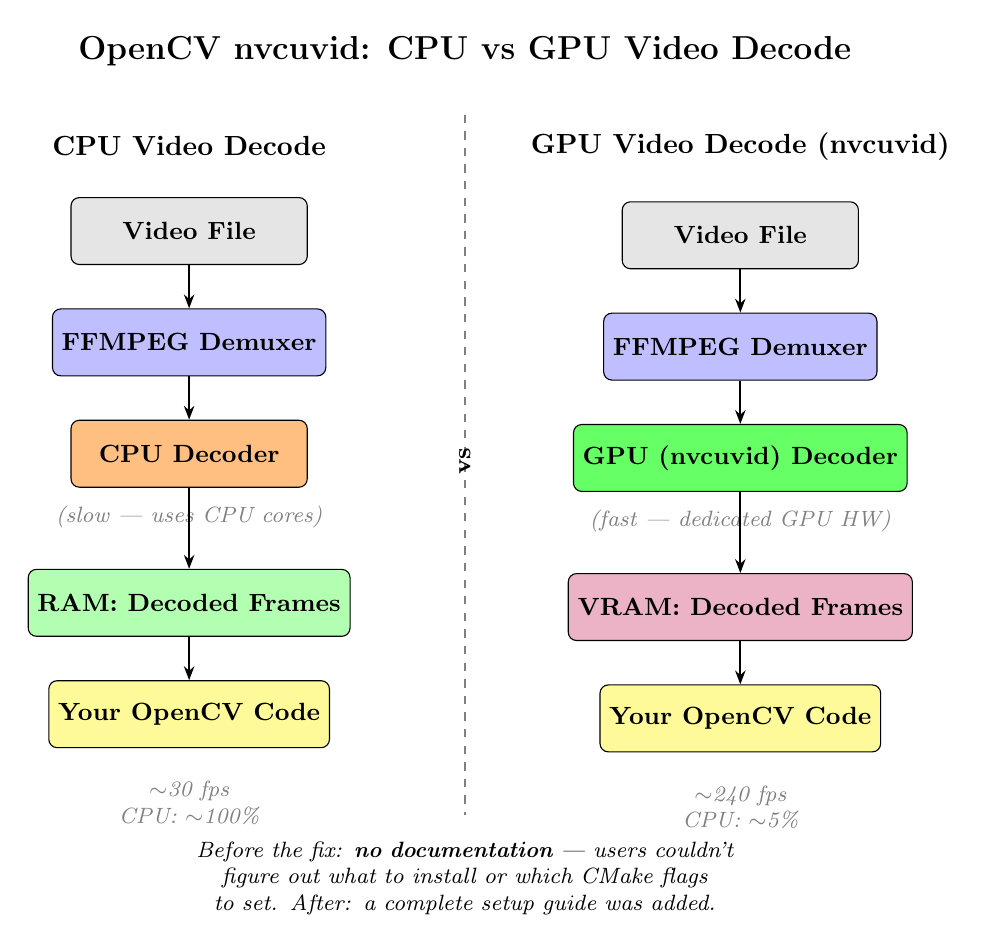
\begin{tikzpicture}[
  node distance=0.55cm,
  box/.style={rectangle, rounded corners=3pt, minimum width=3.0cm, minimum height=0.85cm,
              text centered, draw=black, font=\small\bfseries},
  arrow/.style={-{Stealth[length=5pt]}, thick},
  header/.style={font=\normalsize\bfseries},
  note/.style={font=\footnotesize\itshape, text=gray}
]

% ---- LEFT column: CPU decode ----
\node[header] (cpu_title) at (0,0) {CPU Video Decode};

\node[box, fill=gray!20,   below=0.4cm of cpu_title] (cpu_file)    {Video File};
\node[box, fill=blue!25,   below=of cpu_file]         (cpu_demux)   {FFMPEG Demuxer};
\node[box, fill=orange!50, below=of cpu_demux]        (cpu_decode)  {CPU Decoder};
\node[note, below=0.1cm of cpu_decode]                (cpu_slow)    {(slow — uses CPU cores)};
\node[box, fill=green!30,  below=0.4cm of cpu_slow]   (cpu_ram)     {RAM: Decoded Frames};
\node[box, fill=yellow!40, below=of cpu_ram]          (cpu_app)     {Your OpenCV Code};

\draw[arrow] (cpu_file)   -- (cpu_demux);
\draw[arrow] (cpu_demux)  -- (cpu_decode);
\draw[arrow] (cpu_decode) -- (cpu_ram);
\draw[arrow] (cpu_ram)    -- (cpu_app);

% CPU performance note
\node[note, below=0.3cm of cpu_app, text width=3cm, align=center]
  {$\sim$30 fps\\CPU: $\sim$100\%};

% ---- Vertical divider ----
\draw[thick, dashed, gray] (3.5, 0.4) -- (3.5, -8.5);
\node[font=\small\bfseries, rotate=90] at (3.5, -4) {vs};

% ---- RIGHT column: GPU decode ----
\node[header] (gpu_title) at (7,0) {GPU Video Decode (nvcuvid)};

\node[box, fill=gray!20,   below=0.4cm of gpu_title] (gpu_file)    {Video File};
\node[box, fill=blue!25,   below=of gpu_file]         (gpu_demux)   {FFMPEG Demuxer};
\node[box, fill=green!60,  below=of gpu_demux]        (gpu_decode)  {GPU (nvcuvid) Decoder};
\node[note, below=0.1cm of gpu_decode]                (gpu_fast)    {(fast — dedicated GPU HW)};
\node[box, fill=purple!30, below=0.4cm of gpu_fast]   (gpu_vram)    {VRAM: Decoded Frames};
\node[box, fill=yellow!40, below=of gpu_vram]         (gpu_app)     {Your OpenCV Code};

\draw[arrow] (gpu_file)   -- (gpu_demux);
\draw[arrow] (gpu_demux)  -- (gpu_decode);
\draw[arrow] (gpu_decode) -- (gpu_vram);
\draw[arrow] (gpu_vram)   -- (gpu_app);

% GPU performance note
\node[note, below=0.3cm of gpu_app, text width=3cm, align=center]
  {$\sim$240 fps\\CPU: $\sim$5\%};

% ---- Title and caption ----
\node[font=\large\bfseries] at (3.5, 1.2)
  {OpenCV nvcuvid: CPU vs GPU Video Decode};

\node[font=\footnotesize\itshape, text width=9cm, align=center] at (3.5, -9.3)
  {Before the fix: \textbf{no documentation} — users couldn't figure out what to install or
   which CMake flags to set. After: a complete setup guide was added.};

\end{tikzpicture}
\end{document}
